\documentclass[aspectratio=169]{beamer} %format: 16:9

\usepackage[american]{babel}

\usetheme{ITD1}
\withoutframelogo

\usepackage{booktabs}
\usepackage{csquotes}
\usepackage{derivative}
\usepackage[
  backend=biber,
  doi=true,
  eprint=false,
  date=iso,
  seconds=true,
  style=alphabetic-verb,
  locallabelwidth=true,
  maxnames = 99,
  %citestyle=alphabetic-verb
]{biblatex}
\renewcommand*{\bibfont}{\footnotesize}

\addbibresource{literature.bib}

\title{An Experimental Analysis of the Influence of the Precision of Parameters in an Artificial Neural Network}

% CHANGE IDX HERE
\subtitle{Natural Computation PS Presentation 05}

\author[D. K., E. R., S. A. S., L. S.]{Denise Katritschenko, Elias Reich, Sayed Abozar Sadat, Lukas Schwaiger}
\institute[\plusshort]{\pluslong\\ Department of Artificial Intelligence and Human Interfaces (AIHI)}
\date[\today]{\today}

\AtBeginSection[]{\fullframe{\insertsectionhead}}

\begin{document}

\frame{\titlepage}

\begin{frame}{DoReFa-Net: Introduction}
  \textbf{Last times:} Impact of quantizing fractional parts of the weights to various decimals, training/inference using fp64/fp32/fp16, \dots\\
  \vspace{0.5cm}
  \textbf{This presentation:}
  \begin{itemize}
    \item Quantization in \textit{all} numerical domains: Weights, Activations, and Gradients.
    \item Consideration of \textit{task complexity} $\rightarrow$ dataset and classes.
    \item \textbf{DoReFa-Net}\cite{zhou2016dorefa}: Low-bit running and training of CNN on ImageNet-scale models.
  \end{itemize}
\end{frame}

\begin{frame}{DoReFa-Net: Selected Ideas}
  \begin{itemize}
    \item \textbf{Different bit-widths:} For Weights, Activations, and Gradients for accuracy/efficiency trade-off.
    \item \textbf{Bit-convolution kernel:} Any $M\times K$-bit dot product becomes AND+popcount operation (or XNOR).
    \item \textbf{Different precisions per tensor:} Typically $W\le A \le G$ (e.g., ImageNet $1\text{W}/2\text{A}/6\text{G}$).
    \item \textbf{Straight-Through Estimator (STE):} Keep normal gradients also through non-differentiable quantizers.
  \end{itemize}
\end{frame}

\begin{frame}{DoReFa-Net: Training Pipeline}
  \begin{enumerate}
    \item \textbf{Forward pass}
          \begin{itemize}
            \item Quantize current weights $W^{full-prec}\xrightarrow[]{f_\omega}W^{bit-width}$
            \item Propagate activations, then quantize them $A^{real-valued}\xrightarrow[]{f_\alpha}A^{bit-width}$
          \end{itemize}
    \item \textbf{Backward pass}
          \begin{itemize}
            \item Back-propagate loss - each gradient block is quantized $G\xrightarrow[]{f_\gamma}G^{bit-width}$
          \end{itemize}
  \end{enumerate}
\end{frame}

\begin{frame}{DoReFa-Net: First \& Last FC Layers}
  \begin{itemize}
    \item Quantizing either layer costs $\approx 0.3$pp on SVHN Model A. Smaller models suffer more (up to $1$ pp).
    \item Paper keeps those layers full-precision (fp32) in ImageNet runs.
  \end{itemize}
\end{frame}

\begin{frame}{DoReFa-Net: Accuracy AlexNet on ImageNet}
  \begin{figure}
    \centering
    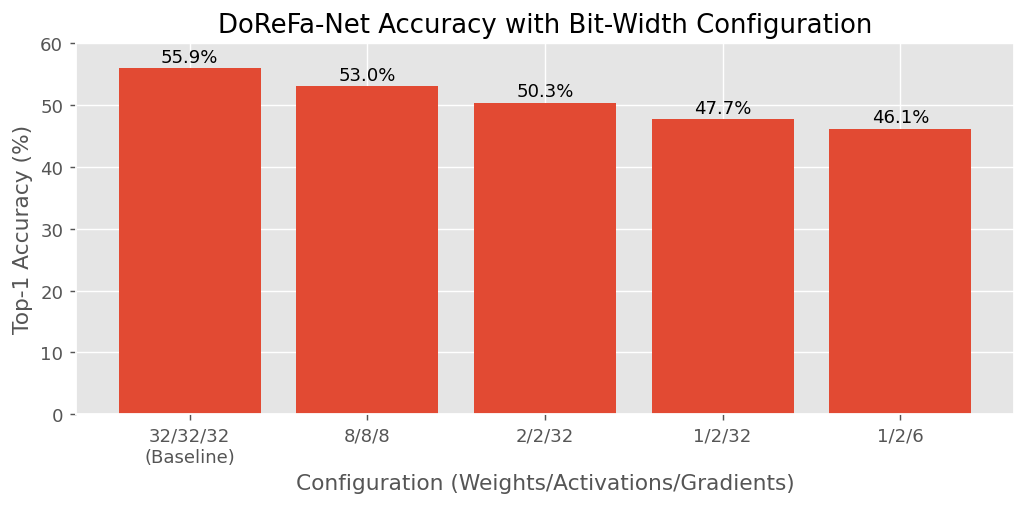
\includegraphics[width=\linewidth]{figures/dorefaRes.png}
    \caption*{\scriptsize Generated bar chart of Top-1 accuracies.}
  \end{figure}
\end{frame}

\begin{frame}{DoReFa-Net: Task Complexity Matters}
  Accuracies of DoReFa-Net on \textbf{SVHN} (10-class house number digit dataset) are very high.\\
  \textbf{Model A} = Full-width 7-layer CNN, trained from scratch with DoReFa quantisation.\\
  \textbf{Model D} = $\frac{1}{8}$-width variant (87.5\% fewer channels $\rightarrow$ network keeps only 12.5\% of the original feature-map width in every convolutional layer). %Example: If Model A has 128 channels in a layer, Model D uses 128x(1−0.875)=128x0.125=16 channels
  \vspace{0.3cm}

  \renewcommand{\arraystretch}{0.85}
  \centering
  \begin{columns}[T,onlytextwidth]
    \column{0.49\textwidth}
    \begin{tabular}{ccc cc}
      \toprule
      $W$ & $A$ & $G$ & Model A & Model D \\
      \midrule
      1   & 1   & 2   & 0.934   & 0.803   \\
      1   & 1   & 4   & 0.968   & 0.846   \\
      1   & 1   & 8   & 0.970   & 0.828   \\
      1   & 1   & 32  & 0.971   & 0.841   \\
      1   & 2   & 2   & 0.909   & 0.808   \\
      1   & 2   & 3   & 0.968   & 0.878   \\
      1   & 2   & 4   & 0.975   & 0.878   \\
      1   & 2   & 8   & 0.975   & 0.866   \\
      1   & 2   & 32  & 0.976   & 0.865   \\
      2   & 1   & 2   & 0.927   & 0.846   \\
      \bottomrule
    \end{tabular}

    \column{0.49\textwidth}
    \begin{tabular}{ccc cc}
      \toprule
      $W$ & $A$ & $G$ & Model A & Model D \\
      \midrule
      2   & 1   & 4   & 0.969   & 0.827   \\
      1   & 3   & 3   & 0.968   & 0.887   \\
      1   & 3   & 4   & 0.974   & 0.897   \\
      1   & 3   & 6   & 0.977   & 0.916   \\
      1   & 4   & 2   & 0.815   & 0.868   \\
      1   & 4   & 4   & 0.975   & 0.915   \\
      1   & 4   & 8   & 0.977   & 0.895   \\
      2   & 2   & 8   & 0.900   & 0.842   \\
      8   & 8   & 8   & 0.970   & 0.955   \\
      32  & 32  & 32  & 0.975   & 0.950   \\
      \bottomrule
    \end{tabular}
  \end{columns}
\end{frame}

\begin{frame}{DoReFa-Net: Learnings \& Outlook}
  \begin{itemize}
    \item Gradient precision (min. 6 bits) is the bottleneck - mixed precision was the next step.
    \item Quantization is not \textit{just for deployment} - it can be applied inside the training pipeline.
  \end{itemize}
\end{frame}

% \begin{frame}{DoReFa-Net: Introduction}
%   \textbf{What are we doing:} Change parameter precision of ANN.\\
%   \vspace{0.5cm}
%   \textbf{This presentation:} Look at the effects of
%   \begin{enumerate}
%     \item lower precision in training and inference.
%     \item lower precision only in inference.
%   \end{enumerate}
% \end{frame}

% \begin{frame}{DoReFa-Net: Network Structure}
%   \textbf{MNIST:} $28 \times 28$ pixel images of handwritten digits.

%   \begin{figure}
%     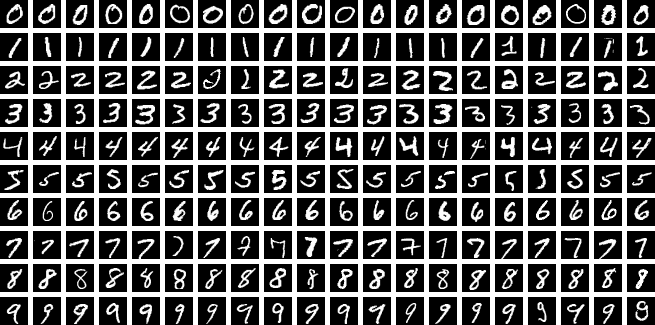
\includegraphics[width=0.7\textwidth]{figures/mnist.png}
%     \caption{MNIST dataset example images~\cite{mnistImage}.}
%   \end{figure}
% \end{frame}

% \begin{frame}{Recap and Today}
%   \begin{itemize}
%     \item Want to optimize the parameters $\omega$ and $b$.
%     \item Need a target $y$ and error metric (loss $L$) to judge the networks predictions
%           $\hat y$.
%     \item Many intermediate results need to be stored for efficient gradient computation.
%   \end{itemize}

%   \begin{align*}
%     L(f(x_1, x_2)) & = (\sigma(\omega^T x + b) - y) ^2 \\
%                    & = (\sigma(a) - y) ^ 2             \\
%                    & = (\hat y - y) ^ 2
%   \end{align*}
%   \begin{alignat*}{3}
%     \pdv{L}{\omega_1} & = \pdv{L}{\sigma} & \cdot & \pdv{\sigma}{a}      & \cdot & \pdv{a}{\omega_1} \\
%                       & = 2(\hat y - y)~~ & \cdot & \odv{}{a}\sigma(a)~~ & \cdot & x_1
%   \end{alignat*}
% \end{frame}

% \begin{frame}{Data and Network Structure}
%   Model evaluation is done with with 5-fold CV.\\

%   \begin{figure}
%     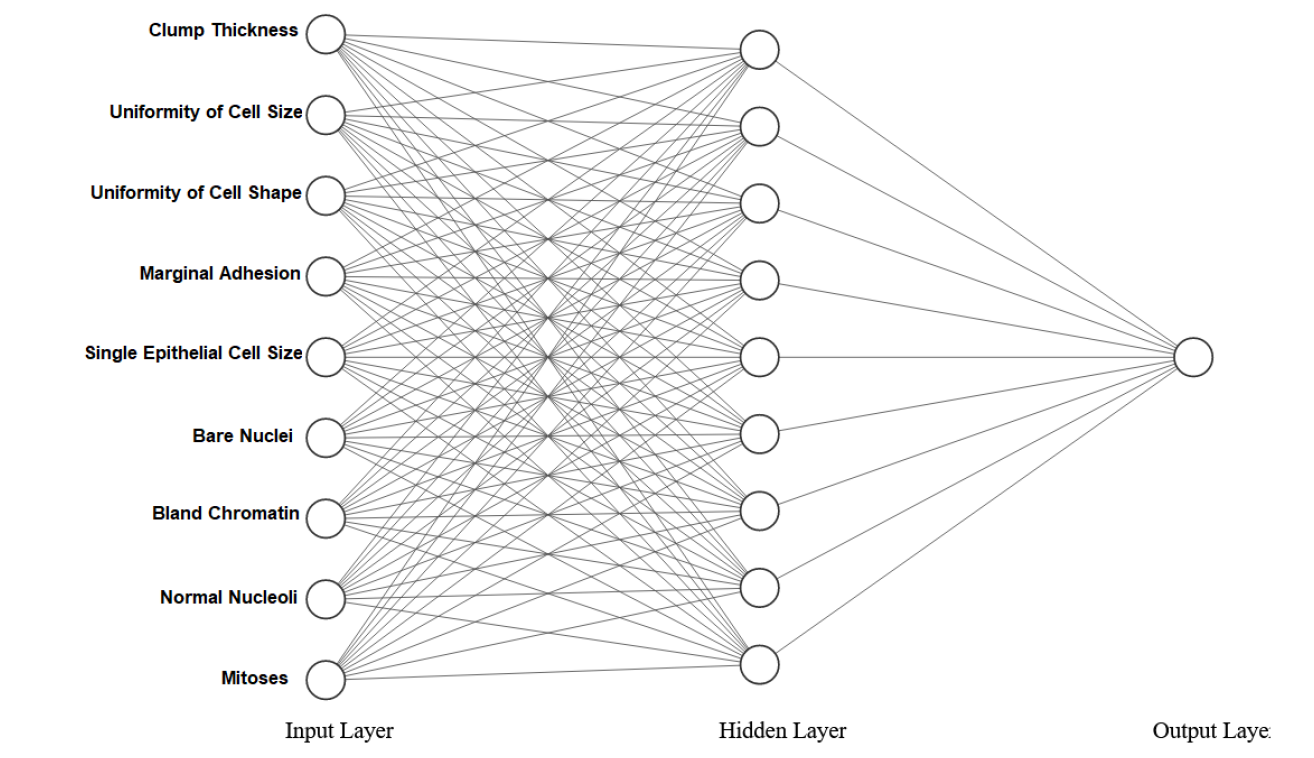
\includegraphics[width=0.8\textwidth]{figures/mlp.png}
%     \caption{Structure of simple NN to classify MNIST numbers.}
%   \end{figure}
% \end{frame}

% \begin{frame}{Results - Training and Inference}
%   \begin{figure}
%     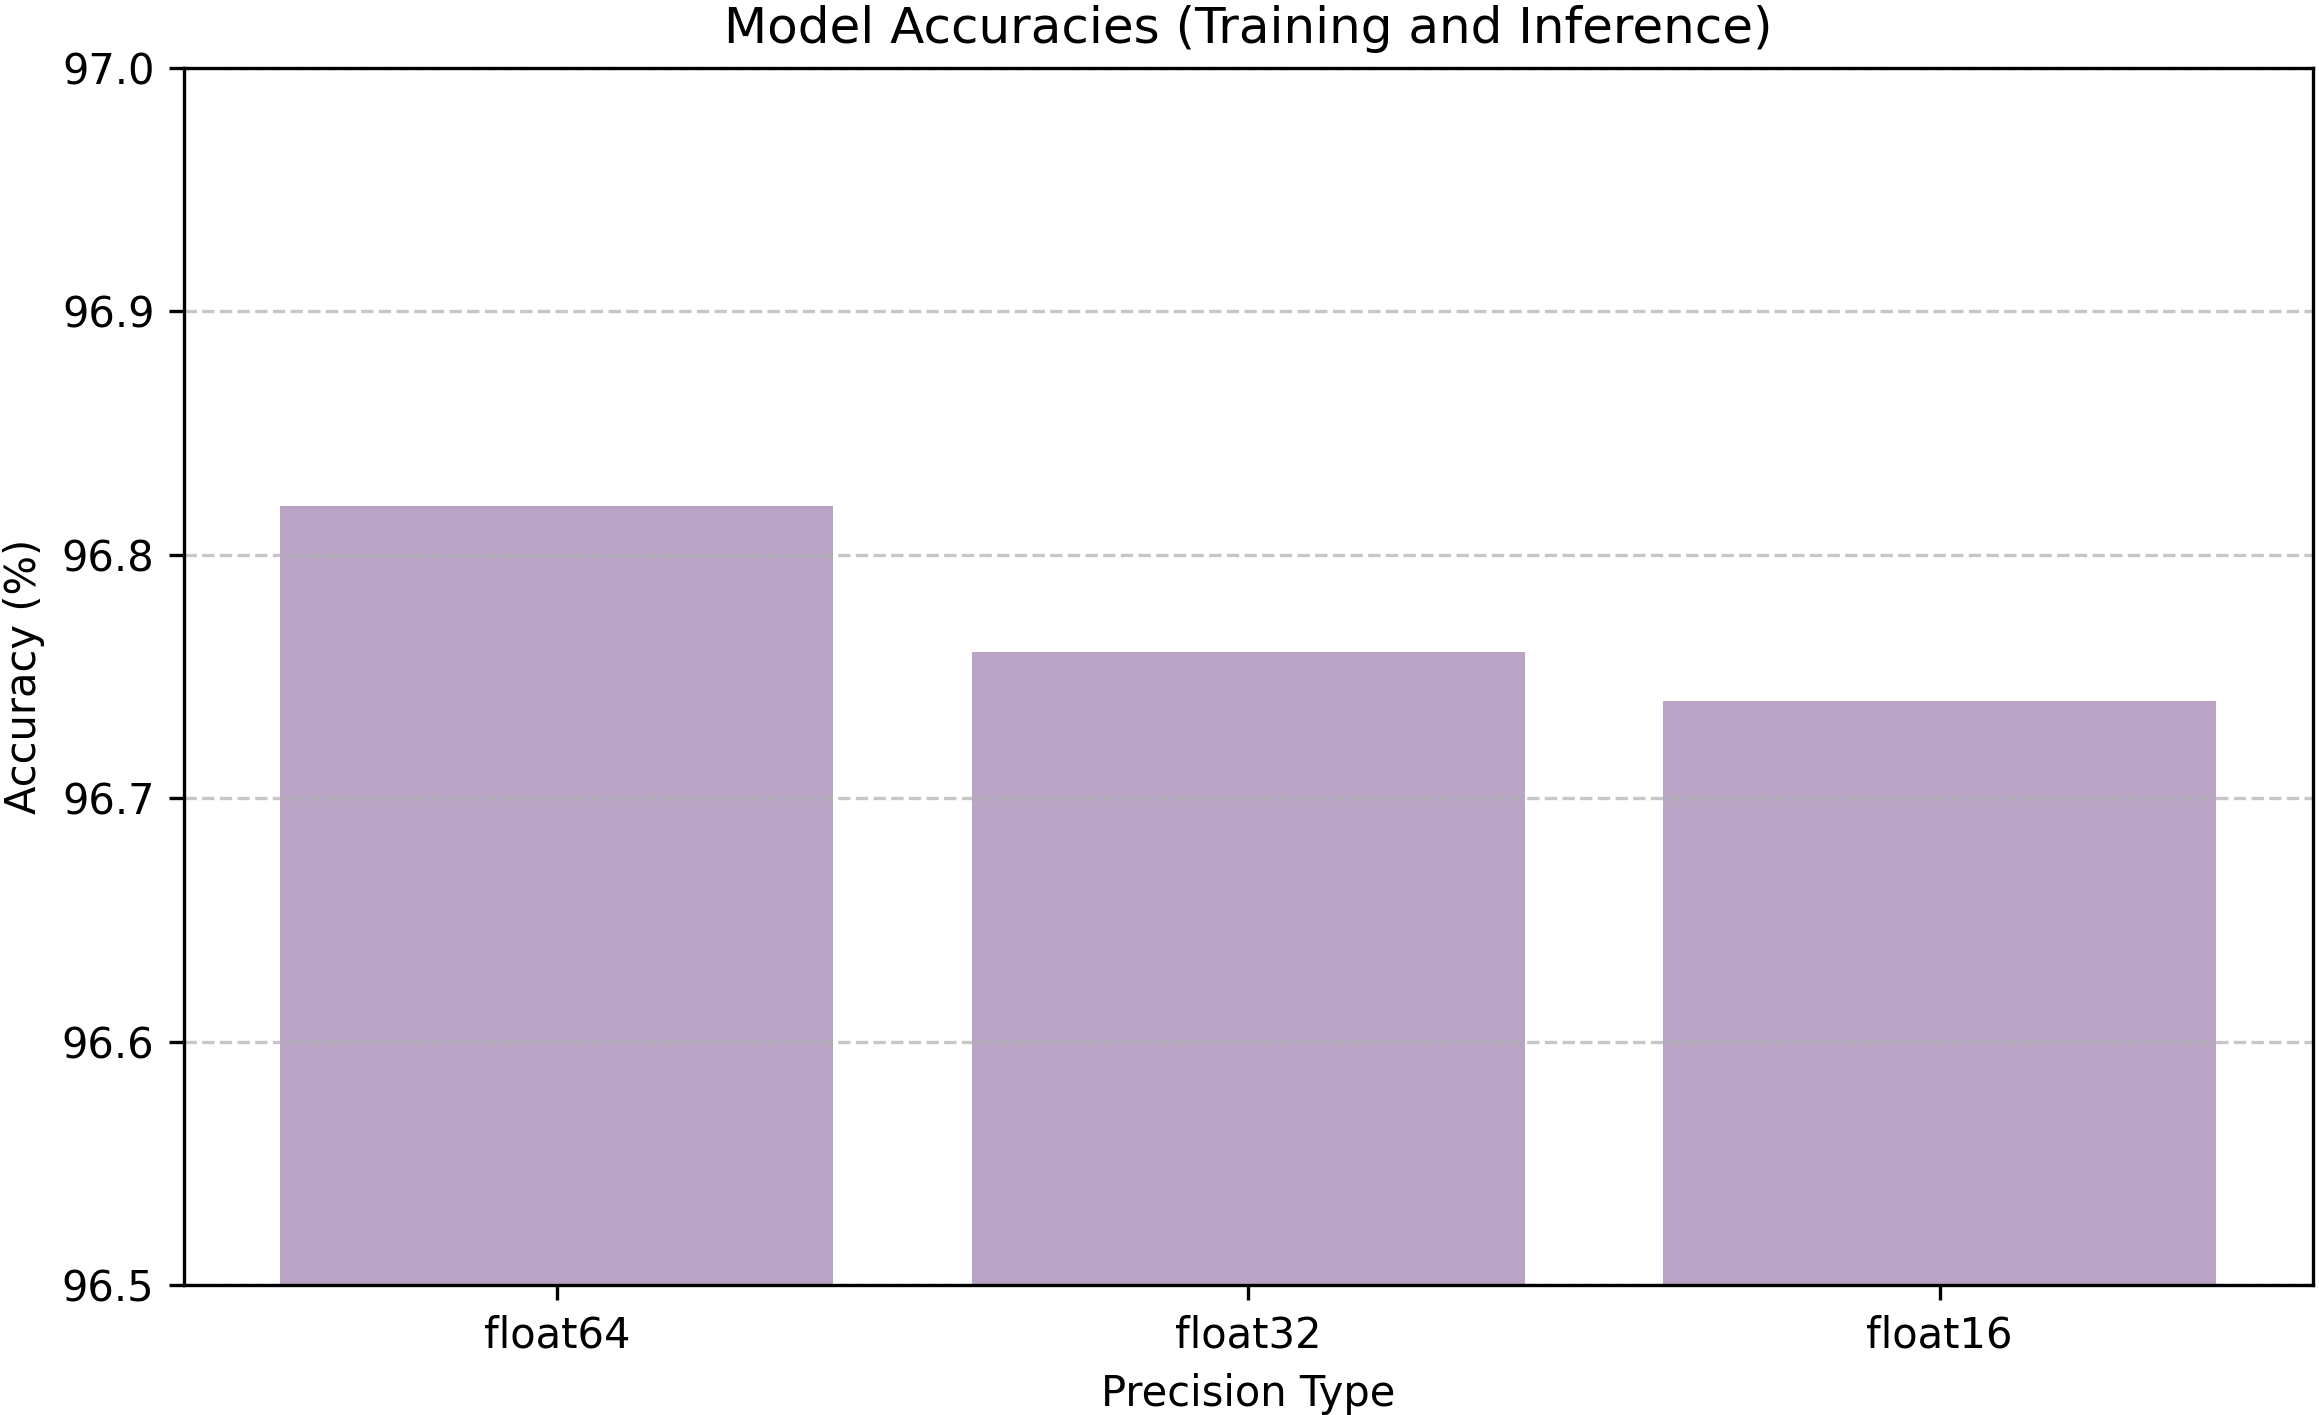
\includegraphics[width=0.7\textwidth]{figures/trainingAndInference.png}
%     \caption{Model accuracies - trained and evaluated at each precision.}
%   \end{figure}
% \end{frame}

% \begin{frame}{Results - Training and Inference Times}
%   \begin{figure}
%     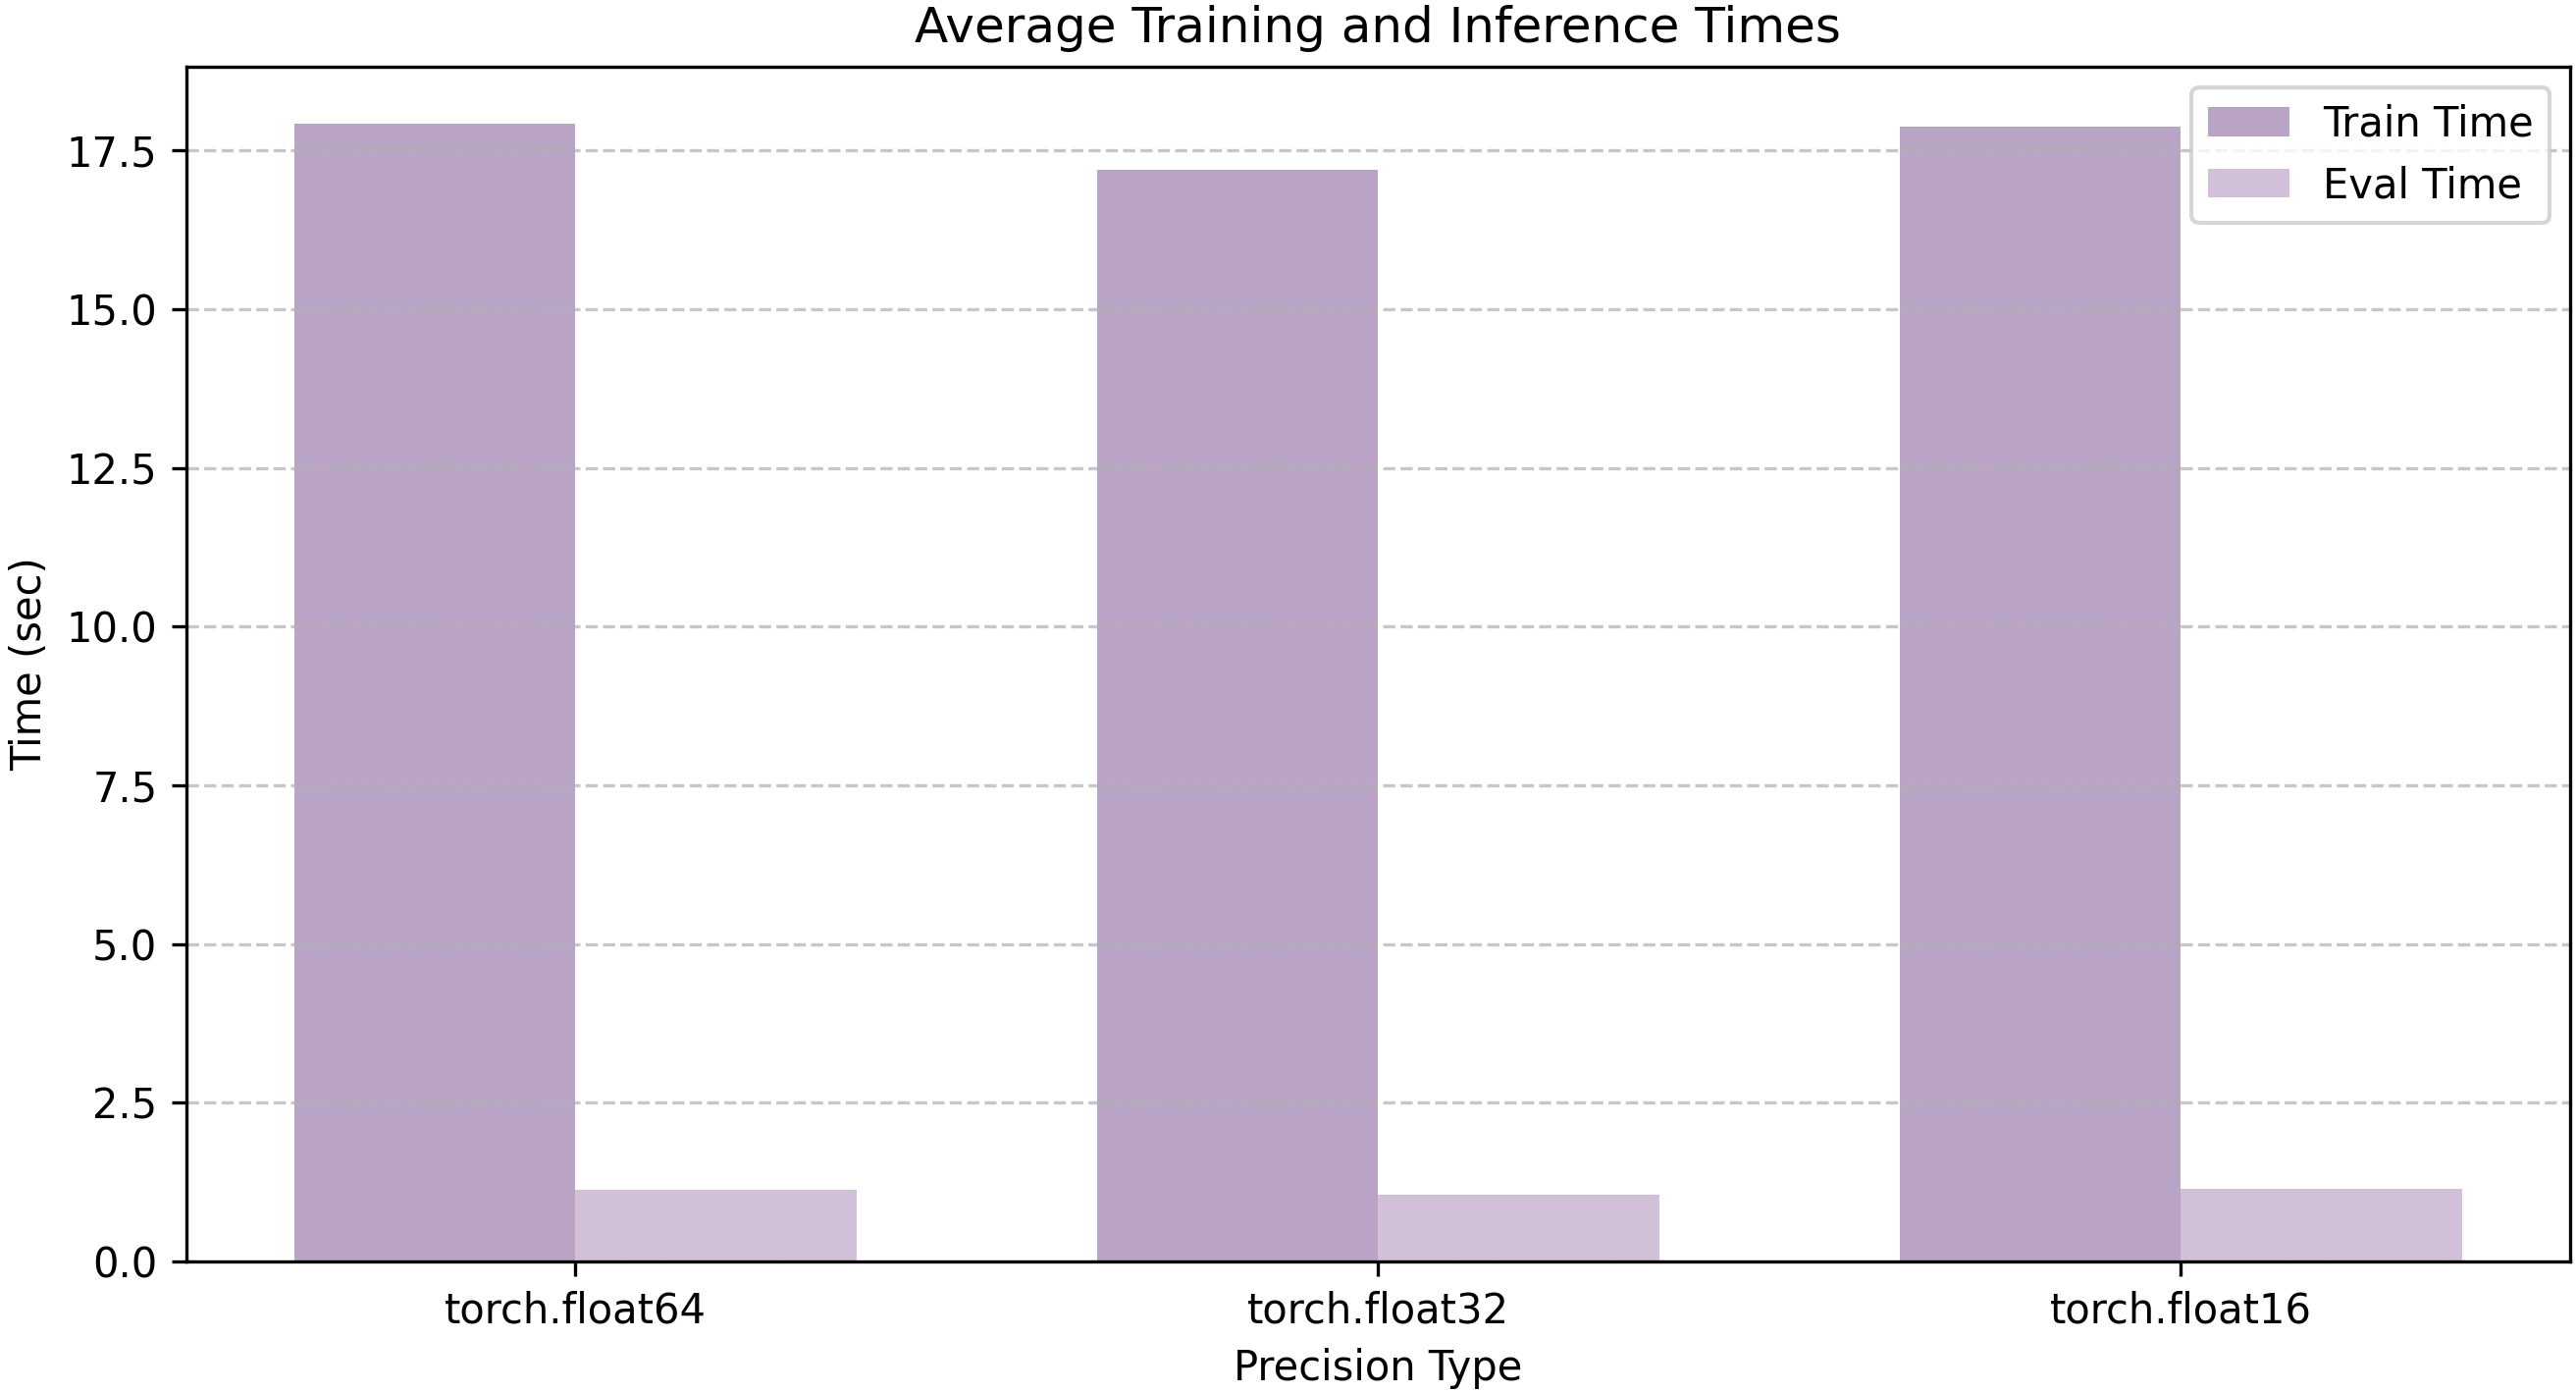
\includegraphics[width=0.7\textwidth]{figures/times.png}
%     \caption{Training and evaluation times.}
%   \end{figure}
% \end{frame}

% \begin{frame}{Results - Inference-Only Testing}
%   \begin{figure}
%     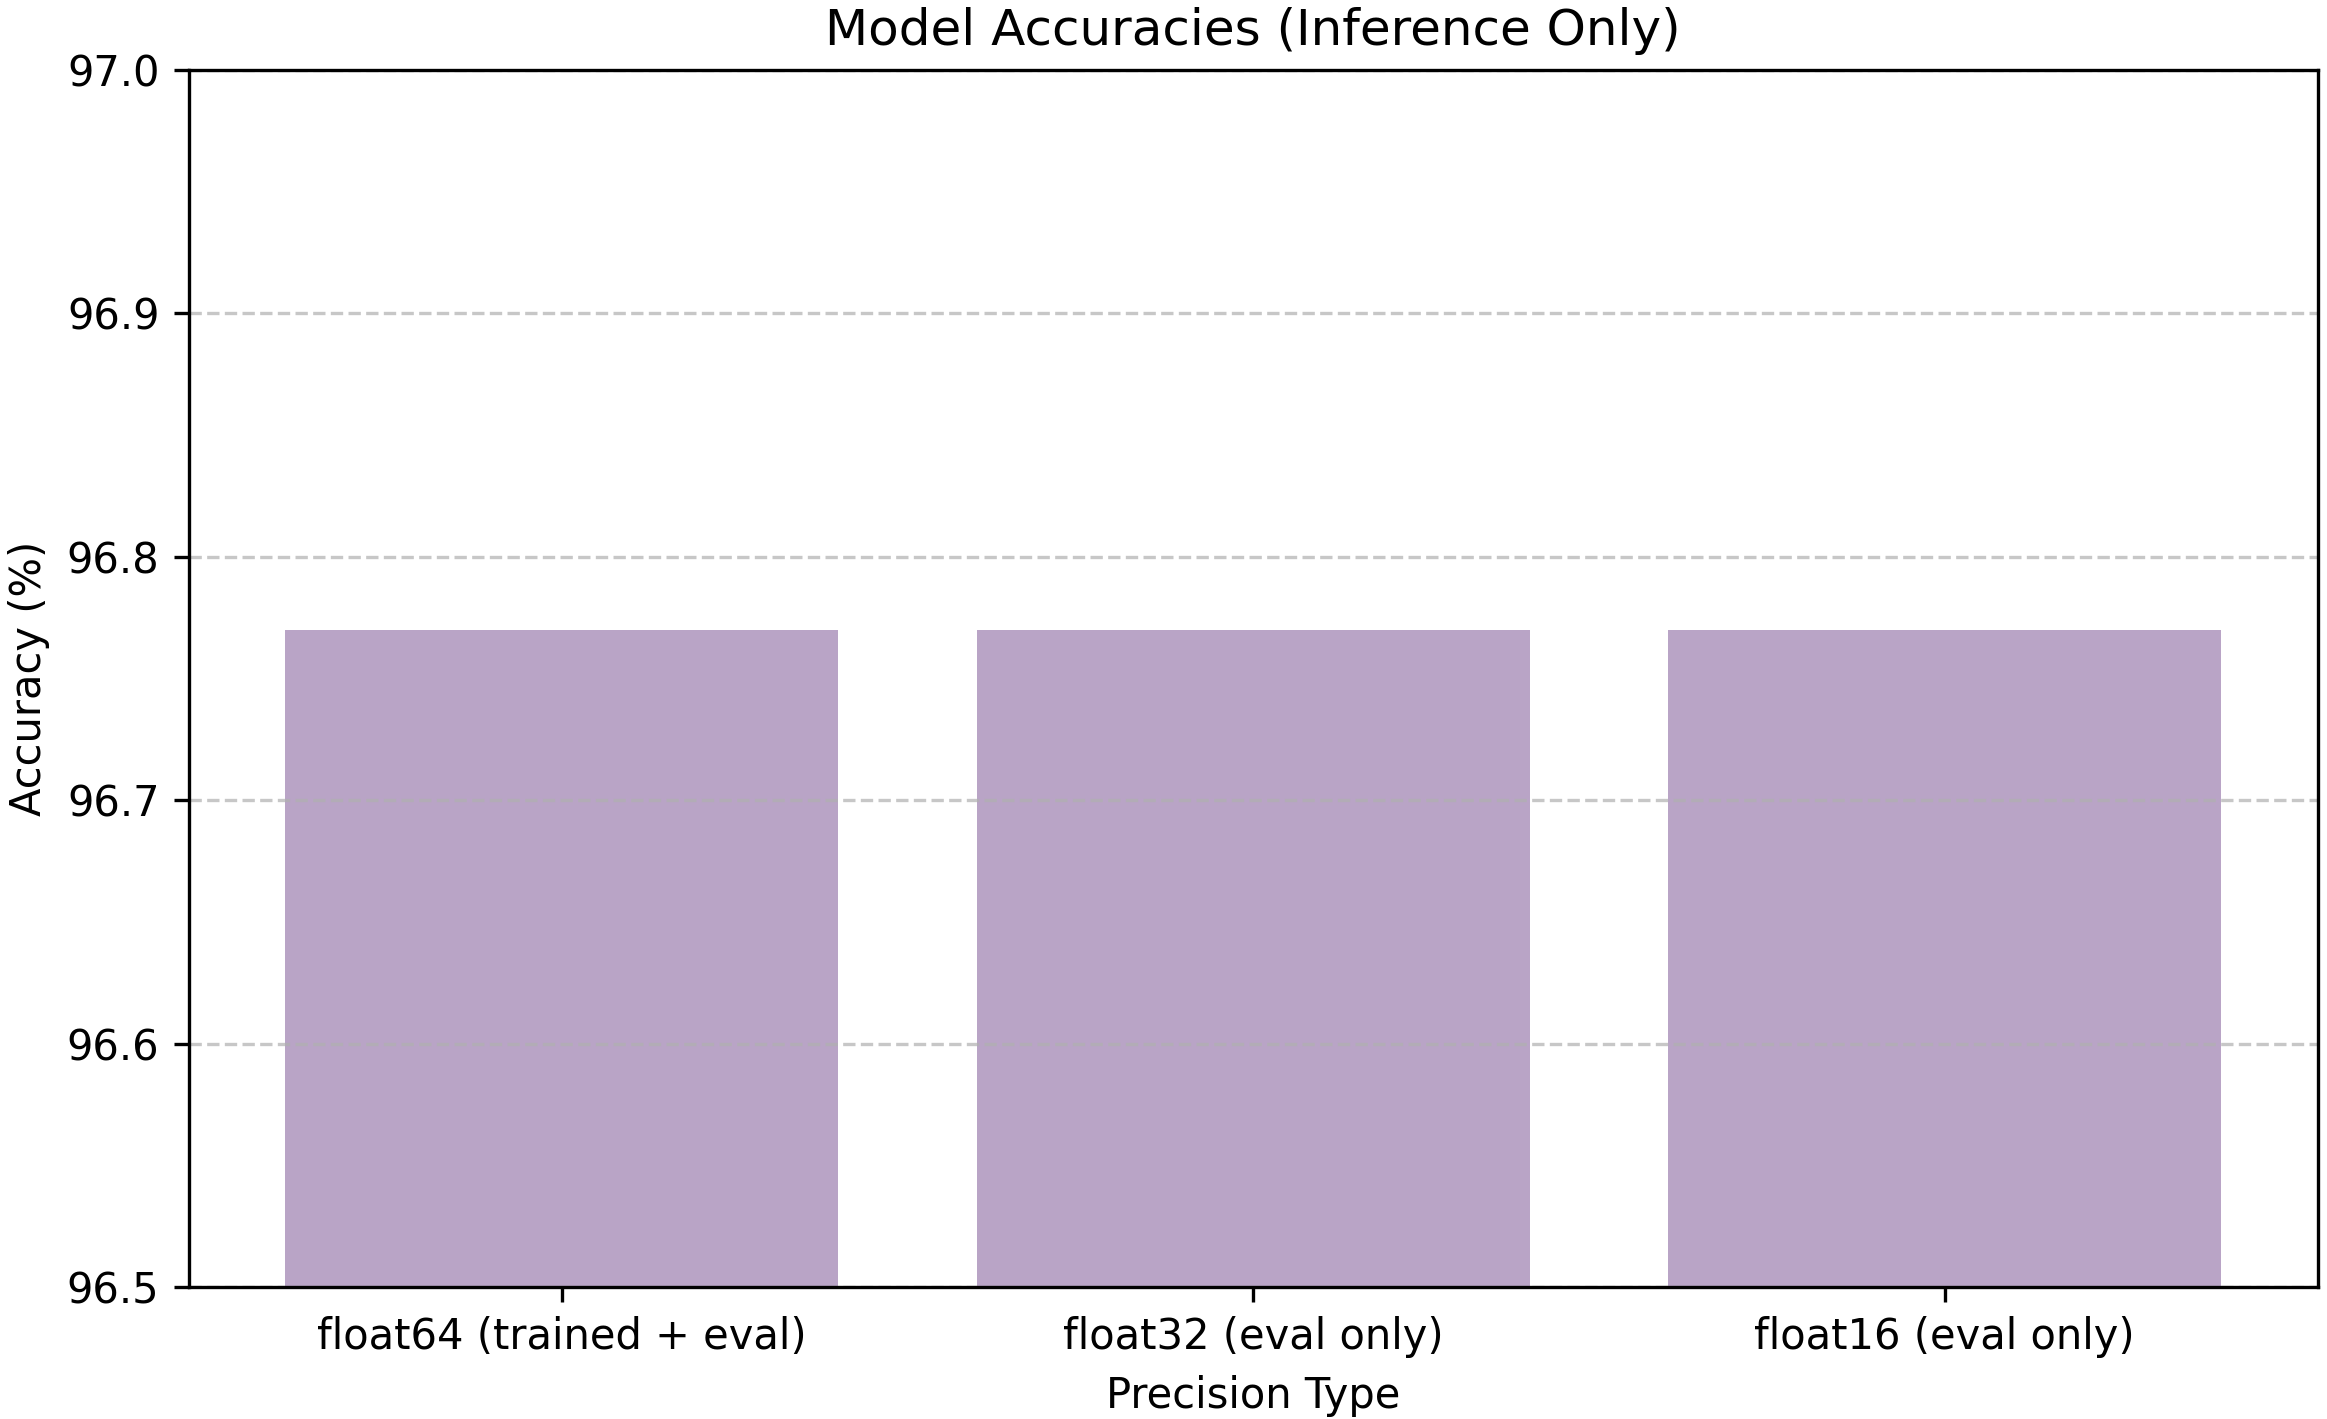
\includegraphics[width=0.7\textwidth]{figures/inferenceOnly.png}
%     \caption{Model accuracies - trained with float64 and post-training precision reduction.}
%   \end{figure}
% \end{frame}

% \begin{frame}{Conclusion and Outlook}
%   \textbf{Interpretation:} Simple task and simple network $\rightarrow$ almost no effets.\\
%   \vspace{0.5cm}
%   \textbf{Next Steps:}
%   \begin{enumerate}
%     \item Reduce precision even further $\rightarrow$ quantize lower than float16 (half
%           precision).
%     \item Mixed Precision Training $\rightarrow$ different bit-widths for different parts
%           of the training process.
%   \end{enumerate}
% \end{frame}

%%%%%%%%%%%%%%%%%%%%

\begin{skipframecount}
  \begin{frame}[allowframebreaks]{References}
    \printbibliography[heading=none]
  \end{frame}

  \appendix
\end{skipframecount}

\end{document}
